\documentclass{article}

\usepackage[utf8]{inputenc}
% Use nameref to cite supporting information files (see Supporting Information section for more info)
\usepackage{nameref,hyperref}
% amsmath and amssymb packages, useful for mathematical formulas and symbols
\usepackage{amsmath,amssymb}
% useful for consistent display and control of units of measurement
\usepackage{siunitx}
% figures!
\usepackage{graphicx}
% for including TODO notes
%\usepackage{todonotes}
% Uncomment next two lines to add line numbers.
\usepackage{lineno}
\linenumbers

\begin{document}

\title{Online Software Allows Ethical Safety-Conscious Design of Terrain Park Jumps}

\author{
  Jason~K. Moore \and
  Bryn Cloud \and
  Mont Hubbard \and
  Christopher~A. Brown \\\\
  J.~K. Moore
  Delft University of Technology\\
  Mekelweg 2, 2628 CD Delft, The Netherlands\\
  j.k.moore@tudelft.nl
  \and
  B. Cloud \& M. Hubbard
  University of California, Davis\\
  One Shields Ave., Davis, CA 95616 USA\\
  becloud@ucdavis.edu,mhubbard@ucdavis.edu
  \and
  C.~A. Brown
  Worcester Polytechnic Institute\\
  100 Institute Rd., Worcester, MA 01609 USA\\
  brown@wpi.edu
}

\maketitle

\begin{abstract}
  Most American snowsport resorts now have terrain parks and decades-long
  epidemiological evidence correlates terrain park use with injuries.
  Engineering design of jumps could reduce injuries by limiting equivalent fall
  heights, which are proportional to dissipated landing impact energy.  No
  evidence refutes making terrain park jumps safer in this way. We discuss case
  studies illustrating that large equivalent fall heights are significant
  factors in traumatic injuries on terrain park jumps. We argue that it is the
  ethical responsibility of engineers to ensure the safety, health, and welfare
  of the public when performing and presenting research on snowsport safety.
  Developing standards and adopting design tools for builders can make jumps
  safer. As an example proactive practice to reduce injuries, we introduce an
  online tool that can evaluate existing jumps as well as design jump profiles
  with safer equivalent fall heights.
\end{abstract}

\section{Introduction}
\label{intro}
%
Impacts with fixed surfaces can cause injury. Greater velocities, perpendicular
to the surfaces, provide greater injury potential due to increased kinetic
energy dissipation. Equivalent fall height (EFH) is a conceptually simple and
familiar measure of impact danger used in safety standards worldwide, from
construction~\cite{OSHA2021} to children's playground
equipment~\cite{Chalmers1996}. EFHs of terrain park jumps can be calculated
using techniques in \cite{Levy2015} from Cartesian coordinates of jump
profiles. These coordinates must include starting points, takeoff ramps, and
landing hills, all along jumpers' paths. Limiting energy dissipation in human
bodies, hence EFH on jumps, reduces likelihoods of injuries and their
severities. EFH should be a primary attribute of jump design. It must be
considered because it is clearly connected to injury risk and can be used to
design and construct safer jumps. In fact, safety research~\cite{Smith2020}
tells us that designing forgiving environments (i.e., limiting EFH at all
possible landing locations) is more effective than forcing behavioral change
(e.g., requiring the jumper to regulate their speed to ensure a landing only in
a small safe region).

Societal costs of jump injuries are discussed here with case studies that
illustrate dangers if EFH is not limited appropriately. We also discuss papers
presented as ski safety research, which attempt to sow doubt about EFH
relevance and snow sport danger, written by authors that regularly provide
expert testimony defending the ski industry in personal injury lawsuits.
Proposals for improved safety are absent in the papers. We present a
user-friendly web application that can facilitate jumping injury reduction by
calculating EFH on current and future jumps.

\subsection{History}
\label{sec:hist}
%
Terrain park jumps are not new. Gradual introduction in the 1980's was
accompanied by increased interest in aerial maneuvers and extreme sports
participation. Jumps have proliferated since and are today nearly ubiquitous.
Roughly 95\% of US ski resorts include terrain parks. Unfortunately, this
growth correlates with injuries. Two early longitudinal studies in the 1980's
and early 1990's~\cite{Deibert1998,Furrer1995} already found significant
increases in head injuries and concussions. Between 1993 and 1997 head injuries
accompanied most skiing and snowboarding deaths~\cite{CPSC1999}. Koehle et
al.~\cite{Koehle2002} stated ``[S]eventy-seven percent of spinal
injuries~\cite{Tarazi1999} and 30\% of head injuries~\cite{Fukuda2001} in
snowboarding were a result of jumps.'' Jackson et al.~\cite{Jackson2004}
determined that by 2004 snow skiing replaced football as the second leading
cause of serious head and spinal cord injuries in America.

These early increasing injury assessments persisted. According to
\cite{Russell2014}, ``between 5 and 27\% of skiing and snowboarding injuries
occur[red] in terrain parks
\cite{Bridges2003,Goulet2007,Moffat2009,Greve2009,Brooks2010,Ruedl2013}''.
Incredibly, at the first Winter Youth Olympic Games more than a third of all
snowboard half-pipe and slope-style competitors were injured~\cite{Ruedl2012}.
Epidemiological research~\cite{Carus2016,Audet2020,Hosaka2020} continues to
show that injuries on terrain park jumps are more likely and more severe than
on normal slopes. Audet et.~al~\cite{Audet2020} provides evidence that skiing
or snowboarding in a terrain park is a risk factor for head, neck, back, and
other severe injuries. Hosaka et. al~\cite{Hosaka2020} concludes that jumping
is a main cause for serious spinal injuries, regardless of skill level, and
suggests that, because spinal injuries incidence  have not decreased over time,
the ski industry should focus on designing fail-safe jump features to minimize
risks of serious spinal injuries. Similar suggestions have appeared in
peer-reviewed literature for more than a
decade~\cite{Hubbard2009,Swedberg2012,Hubbard2012,McNeil2012,McNeil2012a,Hubbard2015,Levy2015,Petrone2017,Moore2018}.

\section{Methods}
\subsection{Equivalent Fall Height}
\label{sec:efh}
%
\emph{EFH}, a common proxy measure for impact danger in industrial safety
standards, is the weight-specific kinetic energy that must be dissipated on
falling impact from height $h$~\cite{Muller1995,Hubbard2009,Gasser2018}.
Initial potential energy $mgh$ is transformed to kinetic energy available to
injure in non-rotating falls. Injury potential can be reduced by controlling
impact circumstances, e.g. impact cushioning, and body orientation,
configuration, and motion; however this energy must still be dissipated. Larger
EFHs require more elaborate measures to reduce injury; reducing EFH does not.

EFH can be interpreted by the general public. People have an intuitive sense of
danger when faced with potential falls from large heights and a strong
experiential common sense for relating fall height to likelihood of injury.
People sense increasing danger associated with falling from larger heights
because injury severity increases with increasing fall height~\cite{Nau2021}.
Ground, second, and third floor falls are about 2.6, 5.1, 8.8~\si{\meter},
respectively~\cite{Vish2005}. The German Society for Trauma Surgery's threshold
for trauma team activation is a fall height of 3~\si{\meter}
\cite{PolytraumaGuidelineUpdateGroup2018}. The US Occupational Safety and
Health Administration has for decades required protection for heights greater
than 1.2~\si{\meter} for general workplace safety~\cite{OSHA2021}.  Chalmers et
al.~\cite{Chalmers1996} argues for 1.5~\si{\meter} maximum fall heights for
playground equipment. The Swiss Council for Accident Prevention makes specific
recommendations for EFHs below 1.5~\si{\meter} for terrain park jumps requiring
basic skills~\cite{Heer2019}.  Even with no standards in Olympic Nordic ski
jumps, typical ``equivalent landing height``~\cite{Gasser2018} is only about
0.5~\si{\meter}.

EFH $h$ of objects is formally defined as
%
\begin{equation}
  h = \frac{v^2}{2g}
  \label{eq:efh_general}
\end{equation}
%
where $v$ is impact velocity and $g$ gravitational acceleration.  Kinetic
energy of objects moving at  velocity $v$  is transformed from potential energy
at height $h$; indisputable, fundamental physics.

Beginning from equation~\ref{eq:efh_general} equivalent fall heights $h$ can be
determined for any surface, i.e., sloped landing profile or shape, after
jumping~\cite{Petrone2017}. The result, neglecting air drag, is
%
\begin{align}
  h = \left[\frac{x^2}{4(x\tan\theta_T - y)\cos^{2}\theta_T} - y\right]
    \sin^{2}
    \left[\tan^{-1}\left(\frac{2y}{x} - \tan\theta_T\right) -
    \tan^{-1}\frac{dy}{dx}\right]
  \label{eq:efh}
\end{align}
%
a function only of takeoff angle $\theta_T$, impact coordinates $(x,y)$
relative to takeoff, and landing surface slope $\frac{dy}{dx}$, but not a
function of takeoff speed~\cite{Petrone2017}. To analyze jumps, one measures
Cartesian coordinates of landing surfaces along jumpers' flight paths and
takeoff angles. Slopes $\frac{dy}{dx}$ are computed from measured coordinates
$(x,y)$. Curvature for the last several meters before takeoffs must be near
zero to avoid unintentional inversion, although this does not influence EFHs.

\subsection{Software and Online Access}
\label{sec:software}
%
We presented the first version of software for designing ski jumps with a
specified EFH in \cite{Moore2018}. It comprises a general-purpose, extensible,
object-oriented software library with tools for 2D skiing simulation. Using
this code, a web application was developed for interactive jump design. The web
application is designed for a non-technical end-user and operable on any
desktop, tablet, or mobile device supporting a web browser.

We have extended the capabilities of the software in version 1.4.0 (March 25,
2021) to assist work described in this paper. New library features automate
calculation of EFH for jump profiles described by a set of Cartesian
coordinates. Additionally, a new ``analysis'' page allows users to upload
measured jump profile coordinates in either a comma separated value or
Microsoft Excel spreadsheet file. The jump is then analyzed and EFHs are
displayed graphically for interactive user manipulation and viewing.
Figure~\ref{fig:web-app-screenshot} shows the web application with one of the
case study jumps (Salvini v. Ski Lifts Inc.) loaded for analysis and explains
its primary features.
%
\begin{figure}
  \centering
  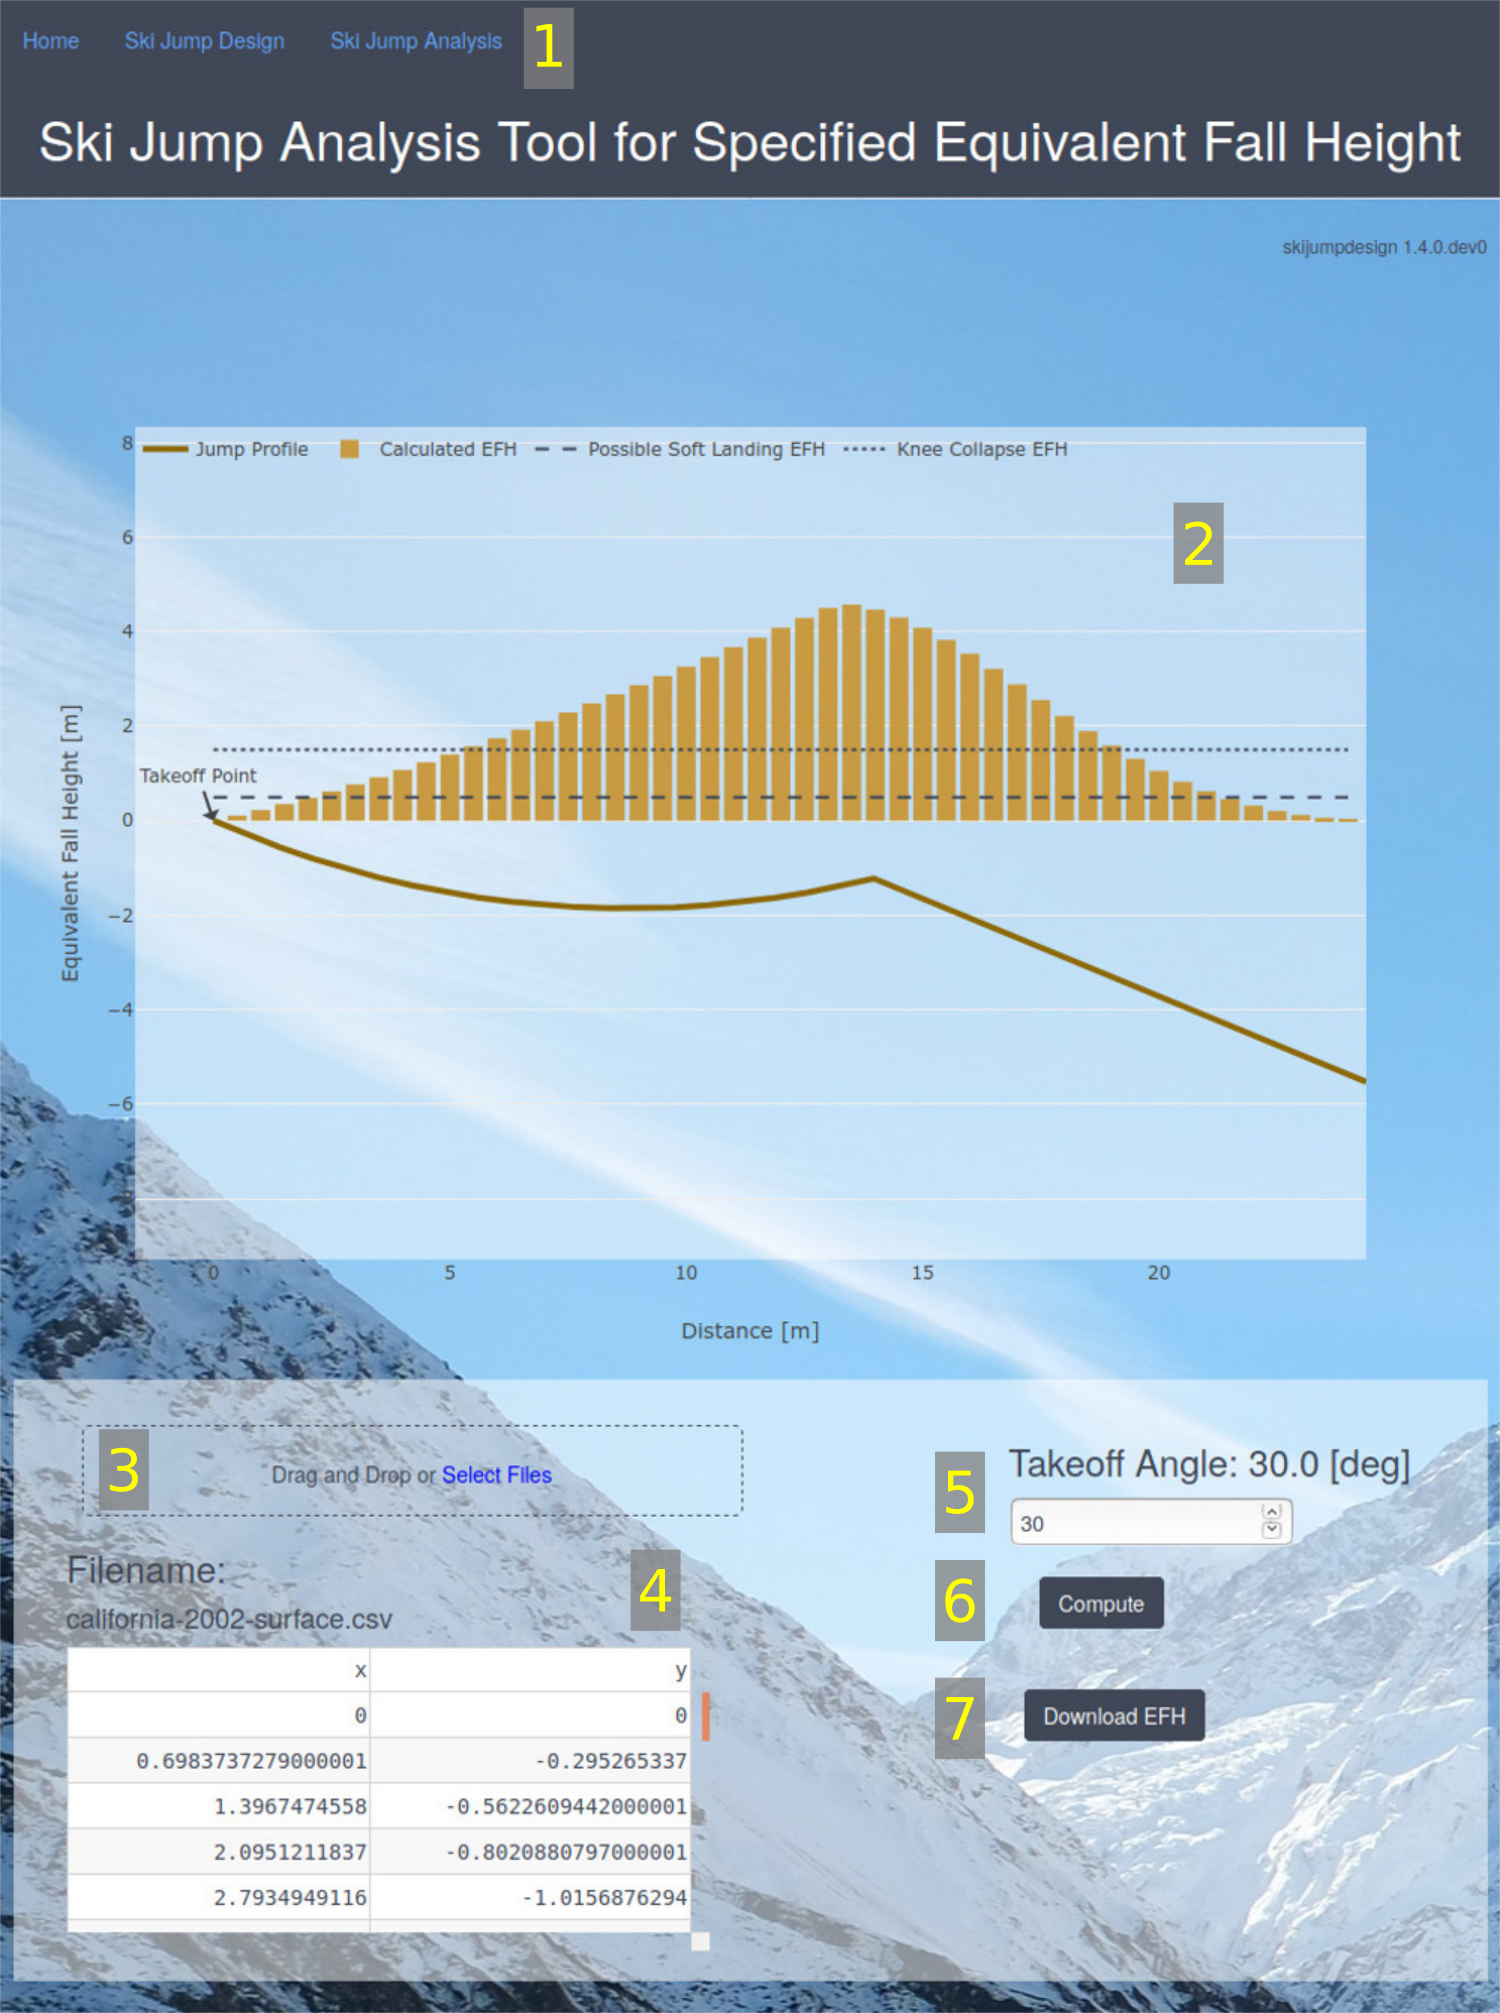
\includegraphics[width=\columnwidth]{figures/web-app-screenshot.png}
  \caption{\textbf{Screenshot of the ski jump design and analysis web app} To
    use the analysis portion of the app, a user selects ``Ski Jump Analysis''
    from the primary menu [1], uploads a .CSV or .XLS file by dragging it onto
    the screen [3], inspects the input data for accuracy in the table [4], sets
    the takeoff angle [5], runs the analysis by pressing the ``Run Analysis''
    button [6], views results in an interactive plot [2], and downloads
     results by pressing the ``Download EFH'' button [7].}
  \label{fig:web-app-screenshot}
\end{figure}

The software is written in Python and directly depends on popular packages
including Cython~\cite{Behnel2011}, matplotlib~\cite{Hunter2007},
NumPy~\cite{Oliphant2006}, pandas~\cite{McKinney2020}, Plotly \&
Dash~\cite{Plotly2015}, pycvodes~\cite{Dahlgren2018},
SciPy~\cite{Virtanen2020}, SymPy~\cite{Meurer2017}, and xlrd. This software is
open source and licensed under the MIT redistribution license. The source code
is distributed on PyPi~\footnote{\url{https://pypi.org/project/skijumpdesign}}.
Users can submit bug reports, feature requests, code improvements, and
additions at the Gitlab
repository~\footnote{\url{https://gitlab.com/moorepants/skijumpdesign}}. The
software library's documentation is hosted via Read the
Docs~\footnote{\url{https://skijumpdesign.readthedocs.io}}.  Basic examples of
using the library are provided in the documentation and this paper's
supplementary materials. We have also made the web application available for
free use online.~\footnote{ \url{http://www.skijumpdesign.info}}

We do not view the software as the definitive ski jump design and analysis
tool, but rather as a foundation. The tool has been released as open-source so
that refinements and modifications are easy and encouraged. The software was
carefully designed with extensibility and modularity in mind. New surface
shapes such as different takeoff ramps are easily added by building upon the
basic surface object using object-oriented programming principles. Similarly,
new skier models can be added that incorporate more complex biomechanical
features and actions. We make use of this flexible software design for the web
application and for the calculations and visualizations presented in the
following section.

\section{Results}
\label{sec:case}
%
In these case studies of American lawsuits, juries ruled for injured
plaintiffs. Negligent jump design and construction contributed significantly to
injuries~\cite{SuperiorCourtSanFranciscoCounty2002,KingCountySuperiorCourt2008}.
Simulations below use methods in \cite{Levy2015}, assuming the same skier mass,
frontal area, and drag coefficient of 75~\si{\kg}, 0.34~\si{\meter\squared},
and 0.821, respectively.

\subsection{Vine v. Bear Valley Ski Company}
\label{sec:vine}
%
In April 2000, Ms.~Vine's lower spine was injured when she landed badly skiing
a jump at Bear Valley in California. The jump shape
(Fig.~\ref{fig:vine-v-bear-valley}) was a common form called a ``table-top''.
Builders intend that jumpers completely clear the table, landing on down-slopes
near a ``sweet spot''. The upper panel of Fig.~\ref{fig:vine-v-bear-valley}
shows the  measured jump surface from accident investigation. Vine landed short
of the knuckle (end of the table-top). This table-top, typically flat and
horizontal, was instead concave, compounding dangers of short landings. At the
11~\si{\meter} landing horizontal distance measured from  takeoff, the surface
sloped upwards approximately 5\si{\degree}. The concave shape emphasizes
detrimental effects of not aligning surface tangents closer to jumper flight
paths at impact.
%
\begin{figure}
  \centering
  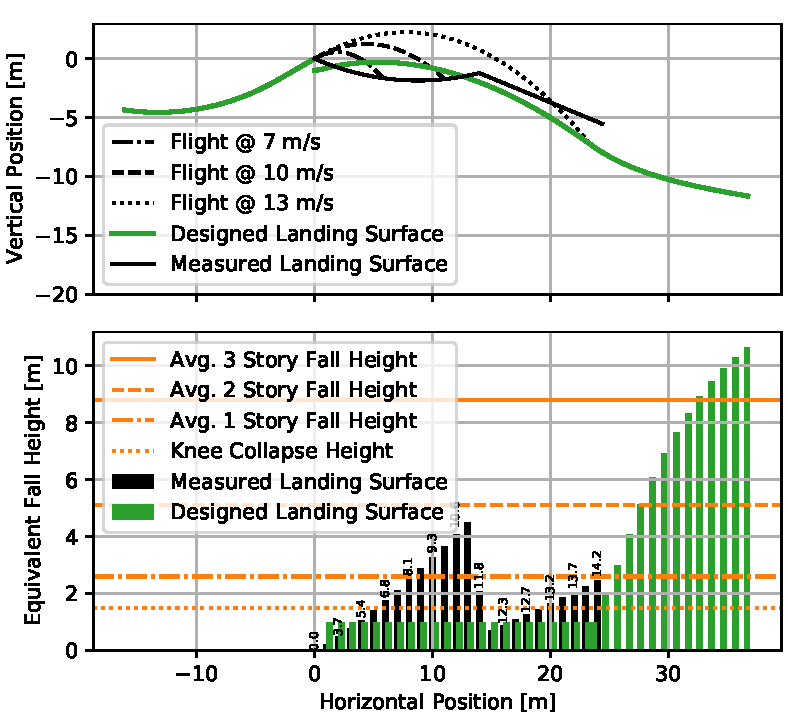
\includegraphics[width=\columnwidth]{figures/vine-v-bear-valley.pdf}
  \caption{\textbf{Bear Valley jump compared to possible safer design}
  Top: Measured landing surface (solid black) and jumper flight paths
  (intermittent black) from measured 30\si{\degree} takeoff angle.  A
  14~\si{\meter\per\second} takeoff speed is used as the design
  speed~\cite{Levy2015} for a comparison jump (solid green) shaped to have
  constant EFH of 1~\si{\meter}.
  Bottom: EFH for both jumps in corresponding colors at 2~\si{\meter}
  intervals. Numbers above bars indicate takeoff speeds required to land at
  that location.
  Intermittent horizontal gray lines indicate increasing relatable fall
  heights: knee collapse, average 1\textsuperscript{st} story fall, and average
  2\textsuperscript{nd} story fall.
  }
  \label{fig:vine-v-bear-valley}
\end{figure}

The lower panel displays EFHs at different landing locations, which are
greatest just short of the knuckle. At the sweet spot, just past the knuckle,
EFHs drop precipitously to  about 1~\si{\meter} although landing in this narrow
region requires jumpers to control takeoff speeds within
1~\si{\meter\per\second}.  Landing at 11 meters, Vine's EFH was almost 4
meters, equivalent to falling from between one and two stories~\cite{Vish2005}.
She had also rotated backward in flight, landed on her lower spine and was
paralyzed. A lower EFH could have decreased likelihood of injury, due to lower
impact forces.

In contrast, landing surfaces designed to have smaller EFHs can be created at
similar cost. The green jump profile in the upper panel of
Fig.~\ref{fig:vine-v-bear-valley} shows a possible jump design,
see~\cite{Levy2015}, of similar size with similar flight times that ensures
constant (smaller) EFHs of about 1~\si{\meter}. The convex shape of this jump
is interestingly close to the original concave table-top  inverted, showing
that convex landing shapes are critically important for limiting EFHs. This
alternative jump design would have lowered impact forces for landings at all
locations. In 2002, the jury ruled in favor of Ms.~Vine, agreeing that Bear
Valley was responsible for providing unsafe jumps.

\subsection{Salvini v. Ski Lifts Inc.}
\label{sec:salvini}
%
In 2004, Mr.~Salvini attempted a table-top jump on skis in the terrain park of
The Summit at Snoqualmie Ski Resort, in Washington state. Salvini overshot the
intended landing location while traveling at typical skiing
speeds~\cite{Shealy2005}, rotated backward during flight and landed on his
back, ultimately suffering quadriplegia. The jury sided with Mr.~Salvini and he
was awarded a judgment of \$14M.

At his landing location of 30~\si{\meter} the EFH exceeded 10 meters,
approximately a 3-story fall. Figure~\ref{fig:salvini-v-snoqualmie} shows the
measured jump surface from the accident investigation.  For takeoff speeds
greater than 13~\si{\meter\per\second}, the lower panel shows that the EFH is
greater than 10~\si{\meter} and growing linearly with larger takeoff speeds.
Severe injury is almost certain in falls this high, especially if landing body
orientation loads the spine, as in this case.
%
\begin{figure}
  \centering
  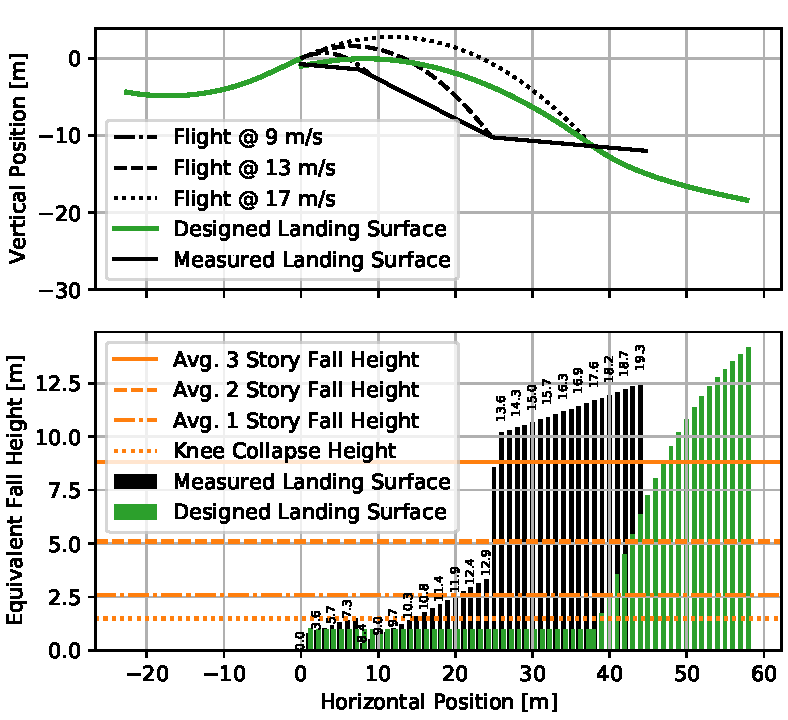
\includegraphics[width=\columnwidth]{figures/salvini-v-snoqualmie.pdf}
  \caption{\textbf{Snoqualmie jump compared to possible safer design}
  Top: Measured landing surface (solid black) and jumper flight paths
  (intermittent black) for measured 25\si{\degree} takeoff angle. The
  16~\si{\meter\per\second} takeoff speed is used as the design speed for a
  comparison jump (solid green) with constant EFH of
  1~\si{\meter}.
  Bottom: Equivalent fall height for both jumps in corresponding colors at
  2~\si{\meter} intervals. Numbers above bars indicate takeoff speed required
  to land at that location.
  Intermittent horizontal gray lines indicate increasing relatable fall
  heights: knee collapse, average 1\textsuperscript{st} story fall, average
  2\textsuperscript{nd} story fall, and average 3\textsuperscript{rd} story
  fall.
  }
  \label{fig:salvini-v-snoqualmie}
\end{figure}

The upper panel also shows a jump profile (green) designed to have a
1~\si{\meter} EFH for all speeds below 16~\si{\meter\per\second}. This profile
requires significantly more snow than the measured jump but alleviates
dangerous impacts. This jump highlights how extreme EFHs can become if jumps
are not properly designed.  Few recreational skiers will jump out three story
windows, snow or not. Injuries are clearly likely. Our internal altimeter tells
us so, but it's not easy to discern when visually assessing a jump's safety.

These two case studies clearly demonstrate that deficient jump landing shapes
have devastating consequences and that engineering analysis and design, based
on laws of mechanics, can be used to shape jump landings that limit EFHs.
Designing jumps this way is based on well-established, centuries-old mechanics
of Isaac Newton and Émilie du Châtelet~\cite{Zinsser2007}, a fundamental of
physics and engineering education. Designing jumps to limit EFHs unquestionably
reduces injury risks by reducing impact energies and associated forces.

\section{Discussion}
\subsection{Moral Imperative}
\label{sec:moral}
%
``Hold paramount the safety, health and welfare of the
public''~\cite{NSPE2019}, is the first canon of engineering ethics. Ethics is
not a matter of opinion and should not be optional. It is the foundation for
engineering. The first canon compels engineers to use their technical expertise
to protect snowsport participants from injuries. Reducing EFHs cannot increase
likelihoods of injuries. Building well designed, safer jumps is no more
laborious than building poorly designed, unsafe jumps. There is no reason not
to control EFHs with good design methods. Nonetheless skiing industries and
their insurance companies are reluctant to adopt and endorse such design
methods, choosing instead to invest in litigation defense rather than
technologies for constructing safer jumps. They hire engineers to profess doubt
on the fundamental physics of EFHs during litigation. Publications cited in
litigation to support these doubts provide little or nothing for the safety,
health, and welfare of the public, that engineers should hold paramount.

In their book ``Merchants of Doubt''~\cite{Oreskes2010}, Oreskes and Conway
have studied this problem more generally. They show that in numerous industries
over the last 60 years, scientific evidence accumulated that commonly accepted
industrial activities were harmful, either to individuals or society. However,
industries had vested interests in continuing practices that were dangerous to
the public, because operational changes would have led to significant,
short-term costs. Examples carefully described and analyzed~\cite{Oreskes2010}
include using DDT, smoking tobacco, producing acid rain from coal-fired power
plants, causing ozone holes from  CFCs, damaging health with second-hand
tobacco smoke, and changing our climate with CO2 emissions. Rather than using
proven science as a basis for changes in practice, strategic responses of
industries have been to ``emphasize the controversy among scientists and the
need for continued research''~\cite{Oreskes2010}.

This same strategy is used by the snowsport industry and its defense experts,
who disparage EFHs.  To sow doubt and counter solid, fundamental, scientific
concepts of landing hill design limiting EFH, defense experts introduce
confounding factors to cloud and confuse basic issues. Consider as evidence
three papers \cite{Shealy2010,Shealy2015,Scher2015} co-authored by well-known
skiing industry defense experts who have testified for snowsport resorts and
their insurance companies. We do not fundamentally question their empirical
findings but we do reject their interpretation of the findings, namely their
conclusion that greater fall height is not a cause of greater injury.

Shealy et.~al~\cite{Shealy2010} conducted an experimental study attempting to
test the hypothesis that takeoff speed is a predictor of the distance from a
jump take-off to landing. They reached the mechanically impossible conclusions
both that there is ``no statistically significant relationship between takeoff
speed and the distance traveled'' and that ``takeoff speed is not a dominant or
controlling factor (in how far a jumper travels)''~\cite{Shealy2010}. These
conclusions were used to question the soundness of analytical mechanical
modeling of jumper flight used in \cite{Hubbard2009,McNeil2012}.

Some of these same authors later vouched for terrain park jump safety. Using
data held by the National Ski Areas Association (NSAA), Shealy et.
al~\cite{Shealy2015} concluded that their ``hypothesis that jumping features
resulted in an increase risk of injury [was] not ...
substantiated.''~\cite{Shealy2015} This is the only study we are aware of with
this conclusion. It is difficult to reconcile it with the voluminous
contradictory research documenting the unique dangers posed by terrain park
jumps in tens of other studies cited both herein and in
\cite{Hubbard2009,Swedberg2012,McNeil2012,McNeil2012a,Hubbard2015,Levy2015,Petrone2017,Moore2018}.
Although NSAA releases yearly totals of resort-related fatalities and
catastrophic injuries, the raw data on which \cite{Shealy2015} was based is not
even publicly available. The data was collected from press releases produced by
the NSAA~\cite{Shealy2015}, which has an inherent conflict of interest, thus
making these results unverifiable.

In a third experimental study (N=13) specifically designed ``to evaluate injury
mitigation potential of surfaces limiting EFH''~\cite{Scher2015}, Scher et al.
clearly show that body orientation, i.e. falling directly on one's head (in all
trials), can cause dangerous cervical spine compression loads~\cite{Scher2015},
even at low fall heights. They report on effects of EFH but only test heights
from \SIrange{0.23}{1.52}{\meter}, committing a similar fault as in
\cite{Shealy2010}, restricting ranges of their independent variables, and
ignoring fall heights known to have caused severe injuries regardless of body
orientation. Yet, they insinuate that EFH has no appreciable effect on
injuries.  The title, ``Terrain Park Jump Design: Would Limiting Equivalent
Fall Height Reduce Spinal Injuries?'' implies that they appear to believe that
falling from greater heights might \emph{not} cause greater injuries. Why
propose such mechanically flawed hypotheses? Sowing doubt on EFH as an
indicator of risk appears to be paramount.

Extending the scope of the findings in these ways are common mistakes, but ones
that should not be made by professional engineers. Fundamental laws cannot be
disproved by these kinds of jumping experiments. If statistical or experimental
results seem in conflict with predictions from classical mechanics, the
problems are most certainly with the statistical or experimental design or
their interpretations, but not fundamental laws of mechanics. Defending
practices that lead to injuries helps prolong these dangerous practices, which
leads to further injuries, clearly contradictory to ethical engineering. Ski
industry defense engineering experts are complicit in the continued societal
damage. As Upton Sinclair wrote ``it is difficult to get a man to understand
something when his salary depends on his not understanding
it''~\cite{Sinclair1994}.

It is not evident that these papers~\cite{Shealy2010,Shealy2015,Scher2015}
``hold paramount the safety, health and welfare of the public''. They are
silent on how their findings can be used to reduce injuries. They obscure a
scientifically fundamental, mechanically irrefutable fact that impacting
surfaces at lower normal velocities is safer. They ``create the appearance that
the claims being promoted were scientific''~\cite[page 244]{Oreskes2010}.
Fundamental laws have made mechanics a science. Findings that contradict such
fundamental laws should be carefully scrutinized and review processes accepting
such articles should be questioned.

Organizations also merchandise doubt. A decade ago, NSAA argued~\cite{NSAA2008}
that, because of rider and snow variability, terrain park jump ``standards are
essentially impossible.'' While it is true that the ``virtually \ldots infinite
number of ways that a given feature may be used by an individual \ldots varying
speed, pop, body movement, takeoff stance, angles of approach, the attempting
of different kinds of maneuvers, landing stance, and the type of equipment used
(skis or snowboard) \ldots create a wide variety of experiences for the
users''~\cite{NSAA2008}, none of these in fact preclude analysis or design.
This was shown clearly in reference~\cite{Hubbard2012} which examined
quantitatively the effects of variations in factors actually involved in the
mechanics: takeoff speed, snow friction, air drag, tail wind, snow melt and
jumper pop. These so-called ``uncontrollable factors'' fell into three groups:
(1) those for which there is zero sensitivity, i.e., an uncontrollable factor
that makes no difference in the ability of the designed jump to deliver the
designed EFH; (2) those for which fairly large parameter variations cause only
insignificant maximum deviations in EFH, and (3) those for which the factor can
be taken into account in the design process itself and its larger effect on EFH
completely eliminated in the unsafe direction. The allegation that design of
limited EFH surfaces is prevented by the complexity of the problem and by the
large number and types of parameter variations away from nominal is false; in
fact the allegation is just more merchandised doubt.

In snowsport injury cases, testifying for injured plaintiffs and testifying
defending corporations are not ethically equivalent. The former attempts to
address problems that cause injuries, holding paramount the public's safety,
health and welfare. The latter attempts to defend practices that might have
contributed to the injury, to limit financial losses of corporations. The idiom
``two sides to every question'', is not appropriate in science and
engineering~\cite[page 268]{Oreskes2010}.

Engineers whose scholarly work ignores engineering's first canon of ethics in
favor of merchandising doubt can diminish the scientific integrity of
engineering journals and engineering conferences. Journal editors should
recognize papers primarily intending to cast doubt on good science and
engineering for what they are, tools of insurance companies for defending civil
suits, and reject them. Papers helping to perpetuate dangerous practices do not
belong in engineering journals or conference proceedings.

\subsection{What Can Be Done?}
\label{sec:action}
%
Absolutely, the most important change will be to incorporate rigorous, rational
processes and scientific principles that consider mechanical impact safety into
designing freestyle jumps.  At present a large fraction of, if not most, jumps
in the USA are created in a formulaic way using two straight lines, a
horizontal deck (tabletop) and nearly constant-slope landing region, linked by
a curved knuckle. This design philosophy is recommended in the instructions
provided by the NSAA~\cite{NSAA2015} and is presumably followed by their
members. Although such jumps are simple and thus easy to design, previous
research has shown that jumps with bi-linear geometry have generally poor EFH
behavior~\cite{Swedberg2012}, i.e. that they can have low EFH only in a small
region just past the knuckle (called the ``sweet spot''). In the more recent
version of their freestyle terrain park notebook~\cite{NSAA2015}, the jump
landing area is even termed the ``landing plan'' because it is envisioned to be
planar! There is no reference whatsoever to any concept such as EFH or similar
measure of impact or its effect on safety because the NSAA's strategy is to put
the responsibility for safety fully on the jumper. There is no quantitative
consideration of jump impact safety (e.g. from the point of view of EFH) beyond
seat-of-the-pants experience of the designer. The skiing industry continues to
resist more scientifically-based rational approaches to design, in spite of the
fact that computer aided design (and even computer-assisted fabrication and
maintenance) of snow park jumps (see Figure~\ref{fig:prinoth}) has been
available from snow groomer manufacturers for more than 5
years~\cite{Muigg2019}. The 2015 NSAA reference in~\cite{NSAA2015} still
contained the statement that ``Standards are essentially impossible~\ldots''.
%
\begin{figure}
  \centering
  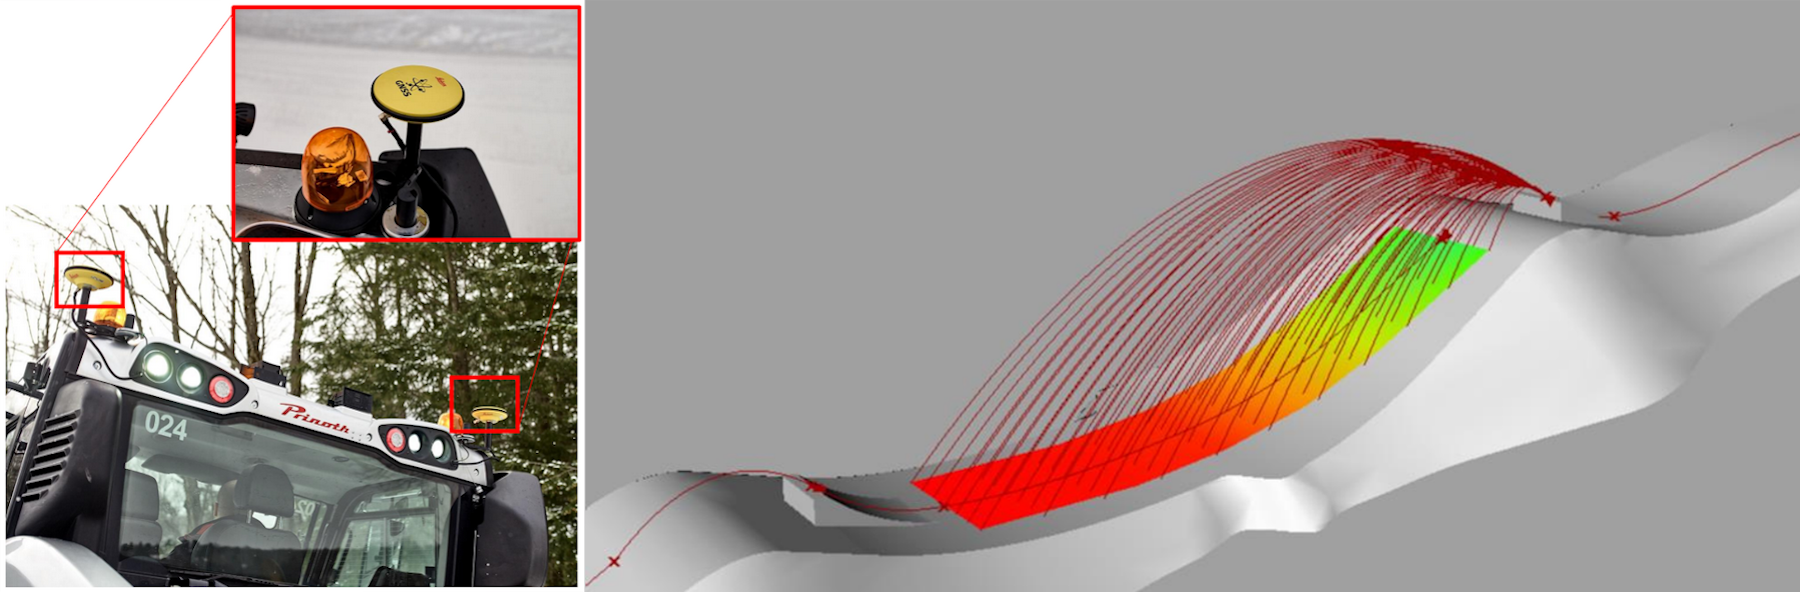
\includegraphics[width=\columnwidth]{figures/prinoth.png}
  \caption{\textbf{Commercial availability of computer-aided design and
    computer-controlled fabrication of snow park surfaces began as early as
    2016.} The right panel shows Prinoth's computer generated 3-D jump landing
    surface with their family of simulated jumper paths, even ones outside the
    central vertical bisecting plane, with the landing surface colored
    corresponding to the EFH incurred by the jumper at that landing point. The
    left panel shows a computer-controlled snow groomer fitted with two GNSS
    receivers that allow real time measurement of their position to an accuracy
    of about 2~\si{\centi\meter}, calculation of the yaw and roll of the
    groomer blade, and precise closed loop control of the snow addition and
    removal process.  Images courtesy of Prinoth, supplier of snow groomers for
  the winter Olympics in China 2022.}
  \label{fig:prinoth}
\end{figure}

Once the jump surface has been designed, the next most important change is to
build accurately what was designed. Presently a dominant fraction of jumps are
simply fabricated by groomer operators, based on perhaps a few measurements of
distances and slopes (deck length, takeoff angle, landing region angle and
length) during the process. But the design concepts are overly simple and do
not incorporate or address quantitative indicators of safety such as EFH. The
introduction of computer controlled grooming (see Figure~\ref{fig:prinoth}),
similar to computer aided manufacturing (CAM), will facilitate precise
construction of more complex designed shapes. These would include the
non-trivial constant EFH surfaces provided by our online ski jump design
software that limit landing impulses to acceptable levels.

Every jumper (and parent of young jumpers) should be able to confirm that a
jump is safe before trying it. Appropriate inspection, evaluation, and
correction of existing jumps, and the design and construction of safer new
jumps should be promoted.  Postings should be required and include EFHs, the
certified inspectors name, and when last inspected.  Inspections should be
frequent enough to ensure that jumps meet the standards, particularly regarding
takeoffs and starting points to prevent inadvertent inversions. Standards need
to be developed that limit EFHs in collaboration between industry and research
engineers to design, build, inspect, maintain, and post safer jumps. An example
of first steps in this area is a terrain park safety guide by the Swiss Council
for Accident Prevention~\cite{Heer2019}.

To complement standards, certification programs are needed for jump building,
inspection, and maintenance. As an example of a successful certification
program, around 1980 ASTM Committee F27 began to develop ski binding standards.
Proponents were led by orthopedic surgeons and academic
researchers~\cite{Bahniuk1996}. Industry argued that standards were impossible
because release value measurement was impossible by ski shops (industry now
makes similar arguments about jumps~\cite{NSAA2015}). Nevertheless
certifications and inspection standards for bindings were developed, which led
to fewer lower-extremity equipment-related injuries~\cite{Bahniuk1996}. But now
no medical professionals and almost no academics remain in F27. Efforts to
create similar standards for terrain park ski jumps began in F27 more than a
decade ago~\cite{SAM2011}, yet no standards have yet been developed. The US
skiing industry, aided by the NSAA, has been successful in delaying the
implementation of standards.

In parallel with standards development, assessing and possibly reshaping
existing jumps to eliminate dangerous EFHs should be an straightforward route
for ski resorts to proactively increase terrain park safety. Accurate enough
measurements of existing surfaces can occur even with simple tools, e.g. tape
measure and digital level, and consume relatively little time and effort per
jump (see supplementary materials for details). Calculation and visualization
of EFHs from these measurements can take some time without a computational
program for calculating EFHs from hill profiles. The user-friendly,
freely-accessible open-source online web application tool that we have made
available for jump designers and builders has almost instantaneous calculation
and visualization steps, solving this problem.

With this software jump builders can easily add safety assessment to their
toolbox, even accessing it from a smartphone or tablet on hills.  We see no
reason that this basic assessment should not be part of jump construction
processes. The only ethical decision is to adopt these methods; saving even one
person from a life of paralysis, or even death, must be worth the relatively
minor inconvenience of shaping jumps using the methods in
reference~\cite{Levy2015}.

\section{Conclusion}
\label{sec:conc}
%
There are, of course, more factors than jump takeoff and landing surface shapes
that contribute to injuries on terrain park jumps. Yet normal impact velocity
can be easily controlled with a properly designed and fabricated landing
surface shape. There is no evidence that decreasing designed EFH increases
injuries in falls; injuries only decrease. Thus we see no reason not to adopt
constant low values of EFH for public-use jump designs. Fabricators of jumps
that are not designed as forgiving environments are negligent. Public safety
must be held paramount to short-term return-on-investment.

The methods implemented in the software illustrated in
Section~\ref{sec:software} provide a starting point for realizing EFH-conscious
designs in terrain parks. We hope to see the design and analysis adopted by
commercial grooming equipment manufacturers so that safety is made integral to
jump design. Our software can grow and evolve through contributions from other
researchers to incorporate many other nuances of injury prevention. We also see
the methods providing a structure for standards development. And minimally, we
see the software as an immediately usable tool for jump fabricators in the
field.

\section*{Acknowledgements}
We thank Rado Dukalski for feedback on the web application and both Yumiko
Henneberry and Lyn Taylor for feedback on the manuscript.

\section*{Declarations}
\begin{description}
  \item[Funding] Not applicable
  \item[Conflict of interest] MH served as a plaintiff's expert witness in the
    two case studies discussed above and in numerous other similar cases since.
    CB testifies occasionally on behalf of plaintiffs in ski and snowboard
    injury cases. He has collaborated with Shealy and C.~D. Mote, Jr., Sher's
    doctoral advisor, on ski safety research, has participated in ASTM F27
    since the 1980s on standards for bindings, boots, and skis, and holds
    patents on ski and snowboard binding designs intended to reduce injuries.
  \item[Availability of data and material] All data is available at
    \url{https://gitlab.com/moorepants/skijumpdesign} and
    \url{https://gitlab.com/mechmotum/ski-jump-analysis-paper}.
  \item[Code availability] The skijumpdesign version 1.4.0 source code is
    archived at \url{https://doi.org/10.5281/zenodo.4637076}. Additionally, it
    and the paper's source code is available at
    \url{https://gitlab.com/moorepants/skijumpdesign} and
    \url{https://gitlab.com/mechmotum/ski-jump-analysis-paper}.
  \item[Author's contributions] JM and MH contributed to the study conception
    and design. Material preparation, data collection and analysis were
    performed by JM and MH. The first draft of the manuscript was written by
    JM, BC, MH, and CB. MH and CB were primarily responsible for drafting
    the parts on merchandising doubt and ethics, respectively. All authors read
    and approved the final manuscript. BC and JM wrote the accompanying
    software.
  \item[Ethics approval] Not applicable
  \item[Consent for publication] JM, BC, MH, and CB consent for publication.
\end{description}

% BibTeX users please use one of
%\bibliographystyle{spbasic}      % basic style, author-year citations
% This one looks good but orders the papers by alphabetical order of last name:
%\bibliographystyle{spmpsci}      % mathematics and physical sciences
% The titles don't show up in this one:
%\bibliographystyle{spphys}       % APS-like style for physics
% None of the three supplied bib styes from Springer match Sports Engineering's guidelines. ieeetr at least orders them correctly.
\bibliographystyle{ieeetr}
\bibliography{references}   % name your BibTeX data base

\end{document}
    